\chapter{Positron Emission\\Tomography (PET)}
\vspace{-40ex}
\begin{flushright}
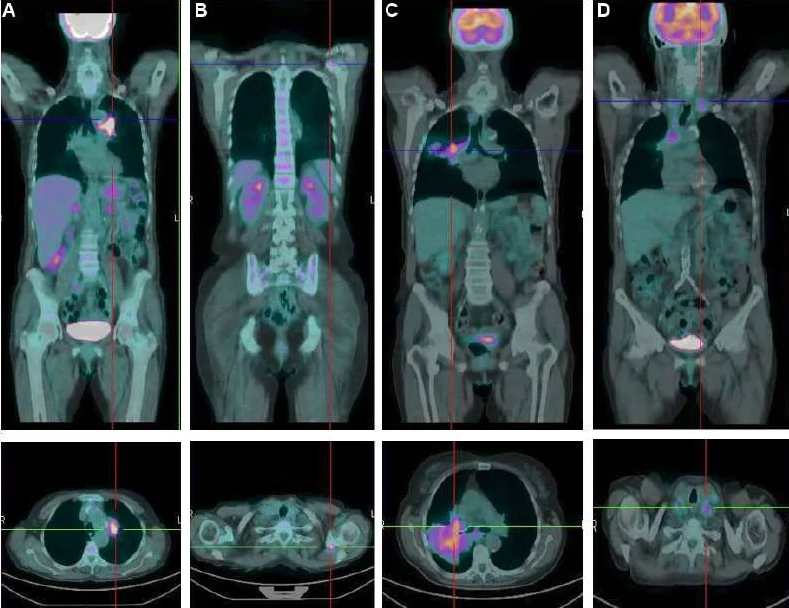
\includegraphics[width=6.5cm]{PET} % https://ksimg.com/wordpress/wp-content/uploads/2022/02/pet-ct.jpg
\end{flushright}

\section{Acquisition}
\begin{itemize}
\item Such as SPECT, PET is a tomographic nuclear imaging system
  \cite{abdulla2025PET}.
\item Employs \popup{annihilation coincidence detection
    (ACD)}{Positron-emitting radioisotopes decay and release a
    positron. This positron travels a short distance, then annihilates
    with an electron from the surrounding tissue, converting their
    mass into two 511-keV photons. These two photons are emitted
    simultaneously and in nearly opposite directions (approximately
    180 degrees apart). PET scanners detect these coincident photon
    pairs using rings of detectors and specialised circuitry. ACD is
    significantly more efficient than collimation and avoids the
    degradation of spatial resolution with increasing distance from
    the detector.} instead of collimation to determine the procedence
  of the radiation that reach the detector.
\item Only uses \popup{positron-emitting radionuclides}{F-18
    fluorodeoxyglucose (FDG) is the most widely used PET
    radiopharmaceutical. Due to their generally short half-lives, PET
    radionuclides often require a cyclotron to be located nearby or
    on-site}.
\item PET scanners are more ``open'' than SPECT scanners because the
  resolution of the images is not so dependent on the distance of the
  camera to the patiend.
\item PET is \popup{more expensive}{A PET/CT system can cost
    approximately twice that of a SPECT/CT system} than SPECT.
\end{itemize}

\section{Clinical applications}
\begin{itemize}
\item As SPECT, it is mainly used to \popup{visualise physiological
    function}{The most common application of PET (especially with F-18
    FDG) is in oncology for differentiating malignant neoplasms,
    staging cancer, and monitoring treatment response.}
  \cite{bushberg2011essential}.
\end{itemize}

\section{Image quality}
\begin{itemize}
\item Compared to SPECT, PET has much higher count rate sensitivity
  and,generating less noise.
\item Therefore, PET images can be reconstructed with much higher
  spatial frequency \cite{abdulla2025NIQ}.
\end{itemize}
